\documentclass[9pt]{article}
 
\usepackage{times}
\usepackage{transparency}
\usepackage[german]{babel}
\usepackage[T1]{fontenc}
\usepackage[utf8]{inputenc}
\usepackage{subfigure}

\screensize{8.5truein}{11truein}
\begin{document}

\title{IPProof - A Generic Network Protocol Packet Generator and Behavior Modeler}

\setbackground{background.png}
\subtitle{\textsf{There is no one-line answer to the question ''How fast can TCP go?'' -- RFC 1323}}


\name{
 \begin{picture}(0,0)
 \put(-90,-130){\includegraphics[scale=0.35]{images/pl-logo.pdf}}
 \end{picture}
}
\footerline{ipproof - a network protocol packet generator}
\email{}
\company{\vspace{4.5cm}\tiny{\textsf{Hagen Paul Pfeifer --- hagen.pfeifer@protocollabs.com}}}
\date{\textsf{22. Juli 2010 -- München}}
\maketitle


%%%%%%%%%%%%%%%%%%%%%%%%%%%%%%
\begin{slide}
\slidetitle{Introduction}{Introduction}
\bi
	\item Core features of ipproof (20\%)
	\item How to utilize and possible application (80\%)
\ei
\end{slide}


%%%%%%%%%%%%%%%%%%%%%%%%%%%%%%
\begin{slide}
\slidetitle{Supported Protocols}{Supported Protocols}
\bi
	\item Network Layer
	\bi
		\item IPv4
		\item IPv6
	\ei
	\item Transport Layer
	\bi
		\item TCP
		\item UDP
		\item UDP-Lite (patch available)
	\ei
	\item ipproof can be used to model application level behavior
\ei
\end{slide}


%%%%%%%%%%%%%%%%%%%%%%%%%%%%%%
\begin{slide}
\slidetitle{Additional Properties}{Additional Properties}
\bi
	\item ipprov provides no analysis functionality
	\item python, ruby, shell scripts in association with tcpdump or pcap traces are required to perform sophisticated analysis,
	ipprov form a vanilla packet generator - not more
	\item Visualization via gnuplot, matplotlib, CairoPlot, octave, R, \dots
\ei
\end{slide}


%%%%%%%%%%%%%%%%%%%%%%%%%%%%%%
\begin{slide}
\slidetitle{Other Features}{Other Features}
\bi
	\item Validation of packet data integrity to check for bit errors (via hamming distance, only payload - no network, transport
	layer header validation)
	\item Windows port (Visual Studio Project file)
	\bi
		\item No UDP-Lite support and other disadvantages due to antiquated network stack
	\ei
\ei
\end{slide}


%%%%%%%%%%%%%%%%%%%%%%%%%%%%%%
\begin{slide}
\slidetitle{Possible Applications}{Possible Applications}
\bi
	\item 
\ei
\end{slide}


%%%%%%%%%%%%%%%%%%%%%%%%%%%%%%
\begin{slide}
\slidetitle{Fundamental Characteristic}{Fundamental Characteristic}
\bi
	\item Bulk Data Emulation
	\item Interactive Emulation
	\item Somewhere in between
	\item Bulk Data
	\bi
		\item unidirectional communication characteristic
		\item Sender transmit data
		\item maximum MSS
		\item TCP congestion mechanism are operative (CWND, SSTRESH, ...)
		\item Receiver is limited to acknowledge data
	\ei
	\item Interactive Data
	\bi
		\item bidirectiol communication characteristic
		\item Sender transmit data, receiver "echo's" the origina data
		\item Small amount of data, a few bytes per packet -  far from link capacity
		\item Nagle algorithm disabled
		\item larger delay between successive packets (user types slower then link delay)
	\ei
	\item Somewhere in Between
	\bi
		\item Send n byte every m microseconds, echoed back after p microseconds q bytes or nothing is echoed
		\item Send 1GB nonrecurring without echo
		\item Send 10MB nonrecurring with a 10kb echo packet (e.g. form some kind of application level acknowledgement)
		\item Send 50 byte data, recuring every minute via UDP to a multicast address
	\ei
\ei
\end{slide}


%%%%%%%%%%%%%%%%%%%%%%%%%%%%%%
\begin{slide}
\slidetitle{Trigger IP Fragmentation/Reassemling}{Trigger IP Fragmentation/Reassemling}
\bi
	\item 
\ei
\end{slide}


%%%%%%%%%%%%%%%%%%%%%%%%%%%%%%
\begin{slide}
\slidetitle{Packet Interarrival Modeling}{Packet Interarrival Modeling}
\bi
	\item Network protocol behavior can be divided into two categories concerning the packet interarrival:
	\bi
		\item Constant arrival time, barely deviations from the packet generation process (e.g. streaming application)
		\item Variable packet generation
	\ei
	\item Last but not least: often the packet arrival differs based on ``environment noise'':
	\bi
		\item Runtime environments with Garbage Collections
		\item Operating system process scheduler latency (e.g. high priority tasks versus low priority tasks)
		\item Egress queuing characteristics (e.g. concurrent data streams, rate limiting egress queueing policy)
		\item Middlebox queueing
		\item Network adapter noise (interrupt moderation, \dots)
		\item Ingress queue
		\item Socket buffer characteristics
		\item Operating system scheduling latency
		\item \dots
	\ei
\ei
\end{slide}


%%%%%%%%%%%%%%%%%%%%%%%%%%%%%%
\begin{slide}
\slidetitle{Receive Buffer Exhausting}{Receive Buffer Exhausting}
\bi
	\item Behaves like an application which forget to read() from the socket (e.g. slow receiver, low priority of receiver
	\item Test to trigger the behavior of zero window probing mechanism of the operating system
\ei
\end{slide}


%%%%%%%%%%%%%%%%%%%%%%%%%%%%%%
\begin{slide}
\slidetitle{Traffic Models}{Traffic Models}
\bi
	\item Long-lived FTP Traffic
	\item Short-lived Web Traffic
	\item Streaming Video Traffic
	\item Interactive Voice Traffic
\ei
\end{slide}

%%%%%%%%%%%%%%%%%%%%%%%%%%%%%%
\begin{slide}
\slidetitle{Modelling Interactive Traffic}{Modeling Interactive Traffic}
\bi
	\item Definition: Interactive TCP Traffic
	\bi
		\item TCP/IP illustrated: The protocols, by W. Richard Stevens and Gary R. Wright
		\item IETF Draft "An NS2 TCP Evaluation Tool" provides some metrics about interactive
		traffic\footnote{http://tools.ietf.org/html/draft-irtf-tmrg-ns2-tcp-tool-00}
		\item Examples: SSH, Telnet, IRC, XMPP (Jabber)
	\ei
	\bi
\begin{verbatim}
[...]
00:00:00.141593 IP 192.168.1.38.47028 > 78.47.222.210.22:   Flags [P.], seq 648:684, ack 889, win 304, length 36
00:00:00.017981 IP 78.47.222.210.22   > 192.168.1.38.47028: Flags [P.], seq 889:925, ack 684, win 91, length 36
00:00:00.000058 IP 192.168.1.38.47028 > 78.47.222.210.22:   Flags [.],  ack 925, win 304, length 0
00:00:00.045855 IP 192.168.1.38.47028 > 78.47.222.210.22:   Flags [P.], seq 684:720, ack 925, win 304, length 36
00:00:00.017156 IP 78.47.222.210.22   > 192.168.1.38.47028: Flags [P.], seq 925:961, ack 720, win 91, length 36
00:00:00.000048 IP 192.168.1.38.47028 > 78.47.222.210.22:   Flags [.],  ack 961, win 304, length 0
00:00:00.783306 IP 192.168.1.38.47028 > 78.47.222.210.22:   Flags [P.], seq 720:756, ack 961, win 304, length 36
00:00:00.017316 IP 78.47.222.210.22   > 192.168.1.38.47028: Flags [P.], seq 961:997, ack 756, win 91, length 36
00:00:00.000054 IP 192.168.1.38.47028 > 78.47.222.210.22:   Flags [.],  ack 997, win 304, length 0
00:00:00.178118 IP 192.168.1.38.47028 > 78.47.222.210.22:   Flags [P.], seq 756:792, ack 997, win 304, length 36
00:00:00.017426 IP 78.47.222.210.22   > 192.168.1.38.47028: Flags [P.], seq 997:1033, ack 792, win 91, length 36
00:00:00.000051 IP 192.168.1.38.47028 > 78.47.222.210.22:   Flags [.],  ack 1033, win 304, length 0
00:00:00.182521 IP 192.168.1.38.47028 > 78.47.222.210.22:   Flags [P.], seq 792:828, ack 1033, win 304, length 36
00:00:00.017470 IP 78.47.222.210.22   > 192.168.1.38.47028: Flags [P.], seq 1033:1069, ack 828, win 91, length 36
00:00:00.000044 IP 192.168.1.38.47028 > 78.47.222.210.22:   Flags [.],  ack 1069, win 304, length 0
00:00:00.170489 IP 192.168.1.38.47028 > 78.47.222.210.22:   Flags [P.], seq 828:864, ack 1069, win 304, length 36
00:00:00.017774 IP 78.47.222.210.22   > 192.168.1.38.47028: Flags [P.], seq 1069:1105, ack 864, win 91, length 36
00:00:00.000055 IP 192.168.1.38.47028 > 78.47.222.210.22:   Flags [.],  ack 1105, win 304, length 0
00:00:00.230487 IP 192.168.1.38.47028 > 78.47.222.210.22:   Flags [P.], seq 864:900, ack 1105, win 304, length 36
00:00:00.017251 IP 78.47.222.210.22   > 192.168.1.38.47028: Flags [P.], seq 1105:1141, ack 900, win 91, length 36
00:00:00.000051 IP 192.168.1.38.47028 > 78.47.222.210.22:   Flags [.],  ack 1141, win 304, length 0
00:00:00.098907 IP 192.168.1.38.47028 > 78.47.222.210.22:   Flags [P.], seq 900:936, ack 1141, win 304, length 36
00:00:00.017255 IP 78.47.222.210.22   > 192.168.1.38.47028: Flags [P.], seq 1141:1177, ack 936, win 91, length 36
00:00:00.000064 IP 192.168.1.38.47028 > 78.47.222.210.22:   Flags [.],  ack 1177, win 304, length 0
00:00:00.118655 IP 192.168.1.38.47028 > 78.47.222.210.22:   Flags [P.], seq 936:972, ack 1177, win 304, length 36
00:00:00.018024 IP 78.47.222.210.22   > 192.168.1.38.47028: Flags [P.], seq 1177:1213, ack 972, win 91, length 36
00:00:00.000060 IP 192.168.1.38.47028 > 78.47.222.210.22:   Flags [.],  ack 1213, win 304, length 0
00:00:00.105917 IP 192.168.1.38.47028 > 78.47.222.210.22:   Flags [P.], seq 972:1008, ack 1213, win 304, length 36
00:00:00.017186 IP 78.47.222.210.22   > 192.168.1.38.47028: Flags [P.], seq 1213:1249, ack 1008, win 91, length 36
00:00:00.000064 IP 192.168.1.38.47028 > 78.47.222.210.22:   Flags [.],  ack 1249, win 304, length 0
00:00:00.398754 IP 192.168.1.38.47028 > 78.47.222.210.22:   Flags [P.], seq 1008:1044, ack 1249, win 304, length 36
00:00:00.017060 IP 78.47.222.210.22   > 192.168.1.38.47028: Flags [P.], seq 1249:1285, ack 1044, win 91, length 36
[...]
\end{verbatim}
	\ei
	\item One keystroke triggers three packets
	\item 192.168.1.38.53758 > 78.47.222.210.22 length 88 length 36
\begin{verbatim}
	0x0000:  4510 0058 a9fa 4000 4006 a1c5 c0a8 0126
	0x0010:  4e2f ded2 d1fe 0016 5ede 73cf 8d75 ff61
	0x0020:  8018 00e3 ef1a 0000 0101 080a 005b 5d29
	0x0030:  70ec 1d99 404b 905f 3000 8b98 7da5 51c0
	0x0040:  5b4c 3a48 6558 f7ad 885c be48 aaa1 b023
	0x0050:  370c 9147 bce4 b82d
\end{verbatim}

	\item 78.47.222.210.22 > 192.168.1.38.53758 length 88 length 36
\begin{verbatim}
	0x0000:  4510 0058 5af8 4000 7606 bac7 4e2f ded2
	0x0010:  c0a8 0126 0016 d1fe 8d75 ff61 5ede 73f3
	0x0020:  8018 005b 9ec6 0000 0101 080a 70ec 2065
	0x0030:  005b 5d29 25b3 3a43 da9b a410 973a 6bea
	0x0040:  791a ab54 64b0 65ca fe21 0b22 541c e981
	0x0050:  409a af26 6d9c 531a
\end{verbatim}

	\item  192.168.1.38.53758 > 78.47.222.210.22 length 52 length 0
\begin{verbatim}
	0x0000:  4510 0034 a9fb 4000 4006 a1e8 c0a8 0126
	0x0010:  4e2f ded2 d1fe 0016 5ede 73f3 8d75 ff85
	0x0020:  8010 00e3 eef6 0000 0101 080a 005b 5d32
	0x0030:  70ec 2065
\end{verbatim}
	
\ei
\end{slide}



%%%%%%%%%%%%%%%%%%%%%%%%%%%%%%
\begin{slide}
\slidetitle{x}{x}
\bi
	\item x
\ei
\end{slide}


%%%%%%%%%%%%%%%%%%%%%%%%%%%%%%
\begin{slide}
\slidetitle{Paket Fragmentierung soll vermieden werden}{Paket Fragmentierung soll vermieden werden}
 \begin{picture}(0,0)
 \put(-530,-490){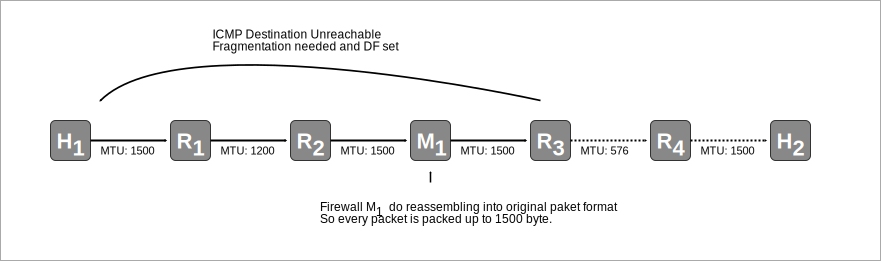
\includegraphics[scale=0.6]{images/blackbox.pdf}}
 \end{picture}
\bi
	\item Fragmentierung und Defragmentierung benötigt zusätzliche Bearbeitungszeit und führt zu höherer Latenz
	\item Fragmentierung verschlechtert das Kontroll/Nutzlast Verhältnis: jedes Fragment bekommt einen eigenen IP Header (dies wirkt sich negativ auf die PER aus).
	\item Fragmentierung bereitet Firewalls, Analyser, ... Probleme.
	\bi
		\item Im Zweifel werden Pakete verworfen wenn die Firewall nicht reassemblieren kann
		\item Wenn die Firewall fragmentiert kann es zu Blackhole Problemen kommen (siehe Beispiel) 
	\ei
	\item Probleme im Zusammenspiel mit Tunneln (z.B. IPIP, Teredo, OpenVPN)
\ei
\end{slide}


%%%%%%%%%%%%%%%%%%%%%%%%%%%%%%
\begin{slide}
\slidetitle{Vielen Dank}{Vielen Dank}
\bi
	\item Viele Dank
\ei
\end{slide}

\end{document}

% vim600: fdm=marker tw=130 sw=4 ts=4 sts=4 ff=unix noet:
